\section{Implementacija apstrakcije}
\label{sec:ImplementationMyAST}

Implementacija prati hijerarhije opisane u poglavlju \ref{chp:MyAST} kroz mehanizam nasleđivanja. Svaki tip čvora je implementiran kao zasebna klasa koja nasleđuje apstraktnu klasu \texttt{ASTNode}. Dijagram klasa koje nasleđuju klasu \texttt{ASTNode} se može videti na slikama \ref{fig:UMLASTNode1} i \ref{fig:UMLASTNode2}. Pored implementacije klasa koje predstavljaju AST čvorove, kreiran je i javno dostupni interfejs za obilazak AST putem obrazca posetilac u implementaciji korišćen za kreiranja graditelja simboličkog izraza od AST koji predstavlja izraz kao i evaluatora takvog AST.

\begin{figure}[h!]
\centering
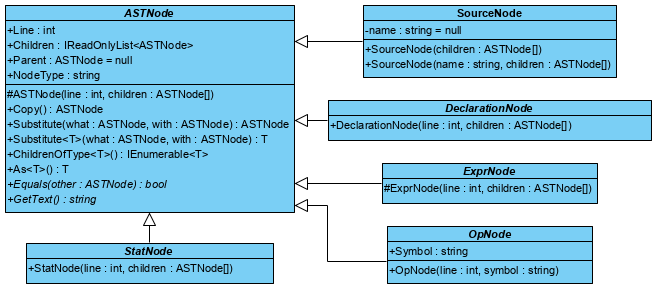
\includegraphics[scale=0.7]{images/uml/ASTNode.png}
\line(1,0){450}\\
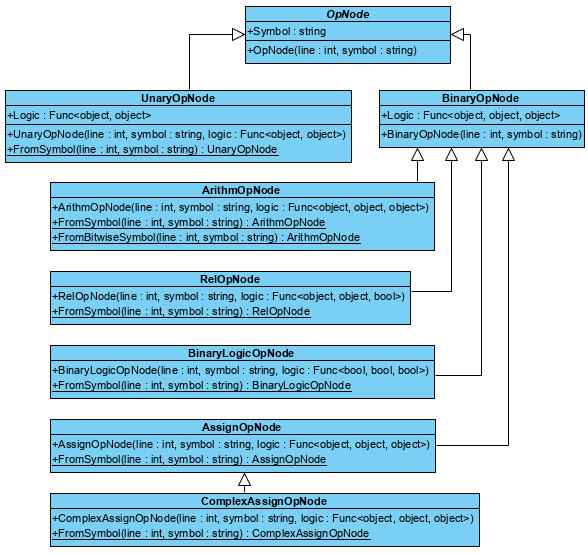
\includegraphics[scale=0.7]{images/uml/OperatorNode.png}
\caption{UML klasni dijagram (deo 1).}
\label{fig:UMLASTNode1}
\end{figure}

\begin{figure}[h!]
\centering
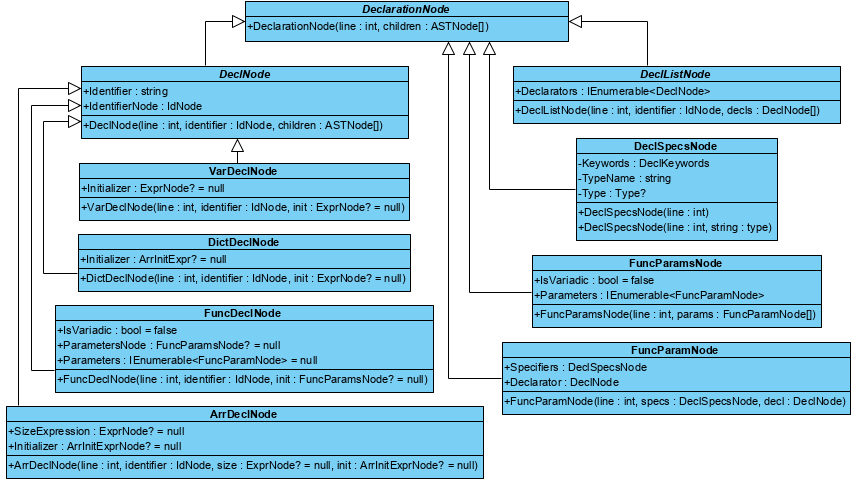
\includegraphics[scale=0.65]{images/uml/DeclarationNode.png}
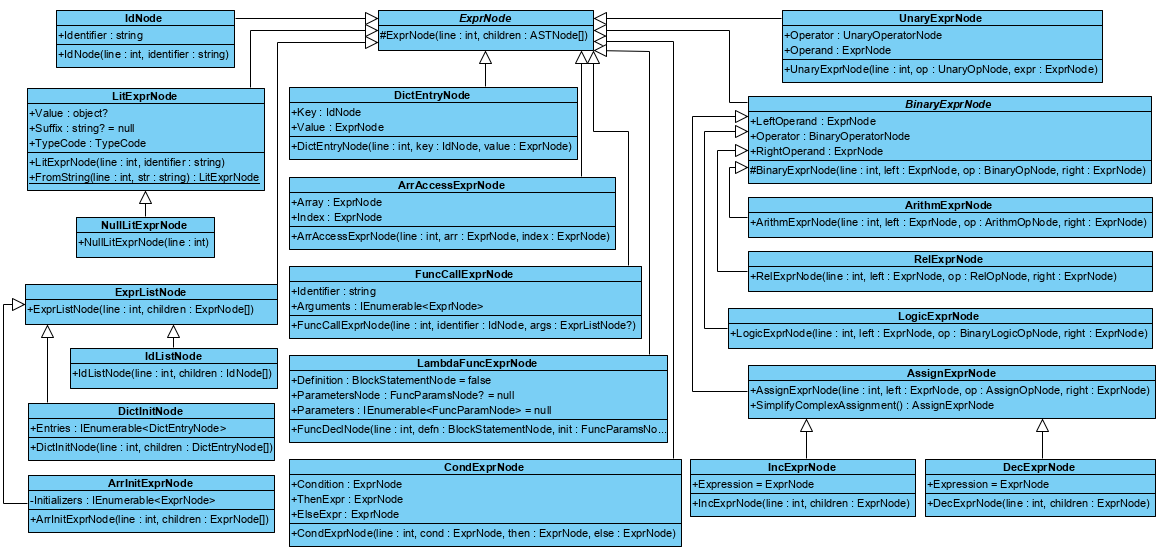
\includegraphics[scale=0.55]{images/uml/ExpressionNode.png}
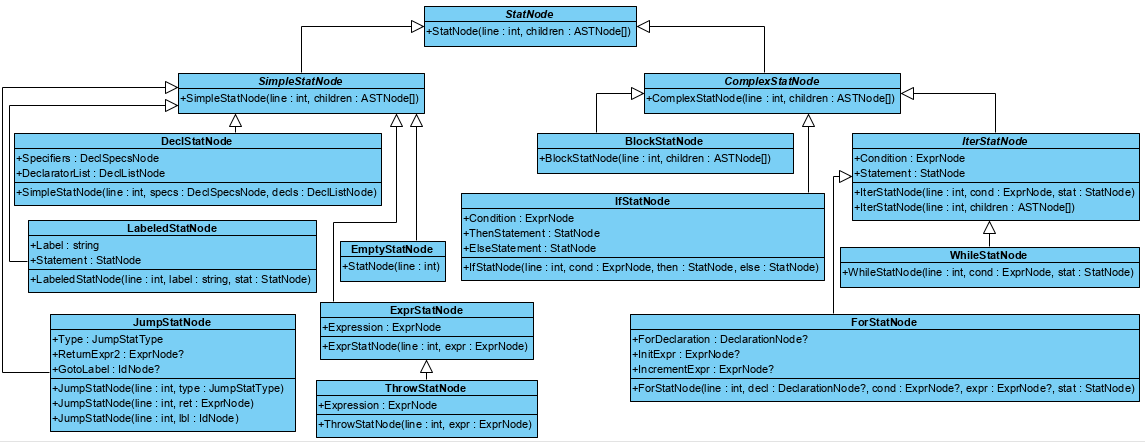
\includegraphics[scale=0.55]{images/uml/StatementNode.png}
\caption{UML klasni dijagram (deo 2).}
\label{fig:UMLASTNode2}
\end{figure}

AST struktura je \emph{imutabilna} --- ne mogu se dodavati ili uklanjati deca čvorovima. Moguće je klonirati AST čvorove ili vršiti zamenu određenog podstabla drugim podstablom ne menjajući original. Svaki AST čvor se može porediti po jednakosti sa drugim AST čvorom po intuitivnoj logici poređenja pruženom kroz predefinisane operatore poređenja.
